\section{Introduction}
\label{sec:intro}  % \label{} allows reference to this 
\subsection{Astrophysical Motivation}

Integrated models of optical observatories are highly beneficial to their design and use\cite{andersen_integrated_2011,Dube2022}. Accurate observatory models permit powerful insight into predicting the as-built performance of a given instrument. However, the accuracy of these models is fundamentally limited by the \added{assumptions made}. To facilitate high-yield scientific observations, astronomical observatories are nominally designed to operate in the diffraction limit where wavefront aberrations are small. Diffraction-limited optical observatories are necessarily modeled with diffraction integrals derived from the Huygens-Fresnel principle to support the wave-like behavior of light. The paraxial and scalar assumptions that angles of incidence are small and that polarization is negligible\cite{goodman17} are made to ease the computational burden on the model. The resultant Fresnel and Fraunhofer diffraction integrals are accurate providing these conditions are met. If the performance of the observatory is limited by a factor outside the assumptions made, then the model will be ignorant of it. \added{An example of this is the linear and shift-invariant assumption imposed on diffraction models of astronomical observatories. Ray aberrations (e.g. coma, astigmatism) have a field dependence, and consequently change across an observatory's field of view. However, diffraction integrals assume shift-invariance. This means that the aberrations do not change across the field of view and a separate ray trace model must be used to capture this effect.}

Integrating optical models from different regimes in physics has become a popular method by which to overcome this limitation. Linking ray trace models to diffraction models in particular can overcome the paraxial and scalar assumption imposed by the Fresnel and Fraunhofer diffraction integrals. \added{In the prior example, to capture the influence of optical aberrations, a new ray trace must be performed and the optical path difference of the rays must be translated to a diffraction model for each point of interest in the field of view.} \added{Similarly, diffraction integrals are incapable of determining the effects of optical polarization. For example,} the Daniel K.~Inoyue Solar Telescope (DKIST) supports a suite of polarimetric instrumentation that is sensitive to the influence of optical polarization. To support this regime of optical physics the scalar assumption is not sufficient, so the polarization state is propagated along geometric ray paths using polarization ray tracing\cite{Chippman15,anche_inprep} to determine the influence of polarization aberrations on the optical beam\cite{Harrington2017}. \added{Modern space telescopes also require integrated models to accurately predict the instrument behavior. For example, } the optical models of the James Webb Space Telescope incorporate the influence of dynamic thermal, structural and optical \added{effects} simultaneously to produce an accurate library of the observatory's jitter\cite{Mather2004}. High-contrast imaging instruments that use coronagraphs, designed to separate exoplanets from diffracted starlight, are in dire need of integrated physical optics modeling from their inception. These \added{coronagraphs} aim to discern targets that are \added{orders of magnitude dimmer than } their host star\cite{Guyon_2006,2015ApJStark,2018Pueyo}. Understanding all sources of error is of paramount importance to the functionality of the instrument.

High-contrast imaging instruments have been successfully deployed on the ground (e.g. SCExAO\cite{Lozi18}, MagAO-X\cite{Males18}, NIRC2\cite{Femenia16}, GPI\cite{Macintosh14}, SPHERE\cite{refId0}) and in space (e.g. NICMOS\cite{thompson_near_1994}, NIRCam\cite{horner_near-infrared_2004,Nircam_exoplanet}) to pursue the direct detection of extrasolar planets, debris, and protoplanetary disks. 
The Decadal Survey on Astronomy and Astrophysics 2020 (Astro2020) recommends pursuing these instruments for a future 6\added{ meter} diameter infrared/optical/visible (IROUV) flagship observatory for the progression of astrophysical sciences\cite{decadal_survey_on_astronomy_and_astrophysics_2020_astro2020_pathways_2021}. 

Presently the optical design of observatories is done in a ray-tracing engine\cite{Howard22,Howard11} (e.g. CODE V, Zemax OpticStudio) because it is more suitable to optimizing the shapes of observatory mirrors. Upon reaching a diffraction-limited optical design, the system is then assumed to be well-represented by a paraxial diffraction model. The wavefront maps produced by the ray trace model of the observatory and the contributions from the imperfect polishing of the observatory mirrors are sent to a \added{linearized }physical optics propagator to examine the image plane electric field in the presence of diffraction from structure in the beam and phase errors on the optics. 

Many tools have been developed to simulate the performance of high-contrast imaging instrumentation. Tiny Tim is one of the first of these widely-used packages used to simulate the Hubble Space Telescope (HST)  instrument point-spread functions (PSFs)\cite{Krist93}. The tool generates aberrated PSFs based on the instrument, observation, and dynamic aberrations for a given observing scenario, enabling highly accurate simulations of the observatory performance. However, it only considers aberrations that are conjugate to the exit pupil of the observatory. This limits the model's ability to capture out-of-pupil effects, like the Talbot effect and speckles from optical surfaces\cite{goodman17}. To capture these effects, optical propagation packages \added{integrate } optical models of observatories by adding Fresnel diffraction to the PSF simulation, enabling the modeling of plane-to-plane diffraction effects. \added{Open-source packages that currently support Fresnel diffraction include:} PROPER \cite{Krist07}, Physical Optics Propagation in PYthon (POPPY)\cite{Perrin12,2016ascl.soft02018P,Doug18}, High-Contrast Imaging in Python (HCIPy) \cite{por2018hcipy}, \added{AOTools\cite{Townson:19}, and prysm \cite{Dube2022,Dube2019}}. Using these tools, near-field diffraction that limits high-contrast imaging can be modeled, and focal-plane wavefront sensing methods can be tested. 

These open-source physical optics propagation tools form the cornerstone of high-contrast imaging instrument modeling and design. The open-source framework means that the codes are accessible to anyone, so the physics are completely verifiable by the scientific community\cite{Allen2021OpenSource}. It is in the scientific community's best interest to continue to develop open-source propagation physics modules to increase the scope of and further integrate our observatory models. 

Commercial optical design codes offer the ability to make diffraction calculations based on ray data, but their physical optics simulation techniques are not as transparent or versatile as the open-source propagation codes that are used to design coronagraphs for astronomical observatories. The current open-source physical optics codes used for observatory modeling are also limited in their scope because of the Fresnel approximation, which is incapable of accurately modeling the field after fast-focusing and highly aspheric surfaces\cite{krist_practical_2010,vanderbei_diffraction_2006}. As observatories get larger, their optics may become faster (i.e. lower $F\#$) and more aspheric to fit within an available volume. Some coronagraph architectures capable of Earth-like exoplanet detection (e.g. phase-induced amplitude apodization\added{, or PIAA }\cite{guyon_phase_nodate}) employ mirrors that apodize the pupil with highly aspheric mirrors, and require tailored propagators in order to be included in physical optics models\cite{krist_practical_2010}. In the regime where the contribution of these surfaces is best represented by a ray trace, a diffraction calculation must be made to appropriately model the optical field at the image plane. \added{To continue the development of integrated optical models, exploring the possibilities and limitations of new propagation techniques is desirable.}

\added{An example of the typical integrated modeling pipeline for astronomical observatories outfitted with coronagraphs is shown in Figure \ref{fig:modeling_flow}. The observatory is typically designed and modeled in ray trace software (e.g. CODE V, Zemax OpticStudio) to accurately model the wavefront in the observatory's exit pupil. Upon finalizing the design, the complex-valued exit pupil is decomposed into a functional representation (e.g. a set of polynomial coefficients, such as the Zernikes\cite{krist_numerical_2015}) and passed to the entrance pupil of a coronagraph model constructed in an open-source, Fourier-based physical optics propagator (e.g. POPPY, PROPER, HCIPy). The front-end model computes the complex field distribution at the coronagraph mask, and then propagates the field past the mask to the image plane. The field is taken by a model of the detector (e.g. EMCCD Detect\cite{Nemati2023}, Pyxel\cite{Pyxel}) to create a simulated raw science image that can be post-processed (e.g. PyKLIP\cite{pyklip}, NMF imaging\cite{nmfimaging}).}

\begin{figure}[H]
	\centering
	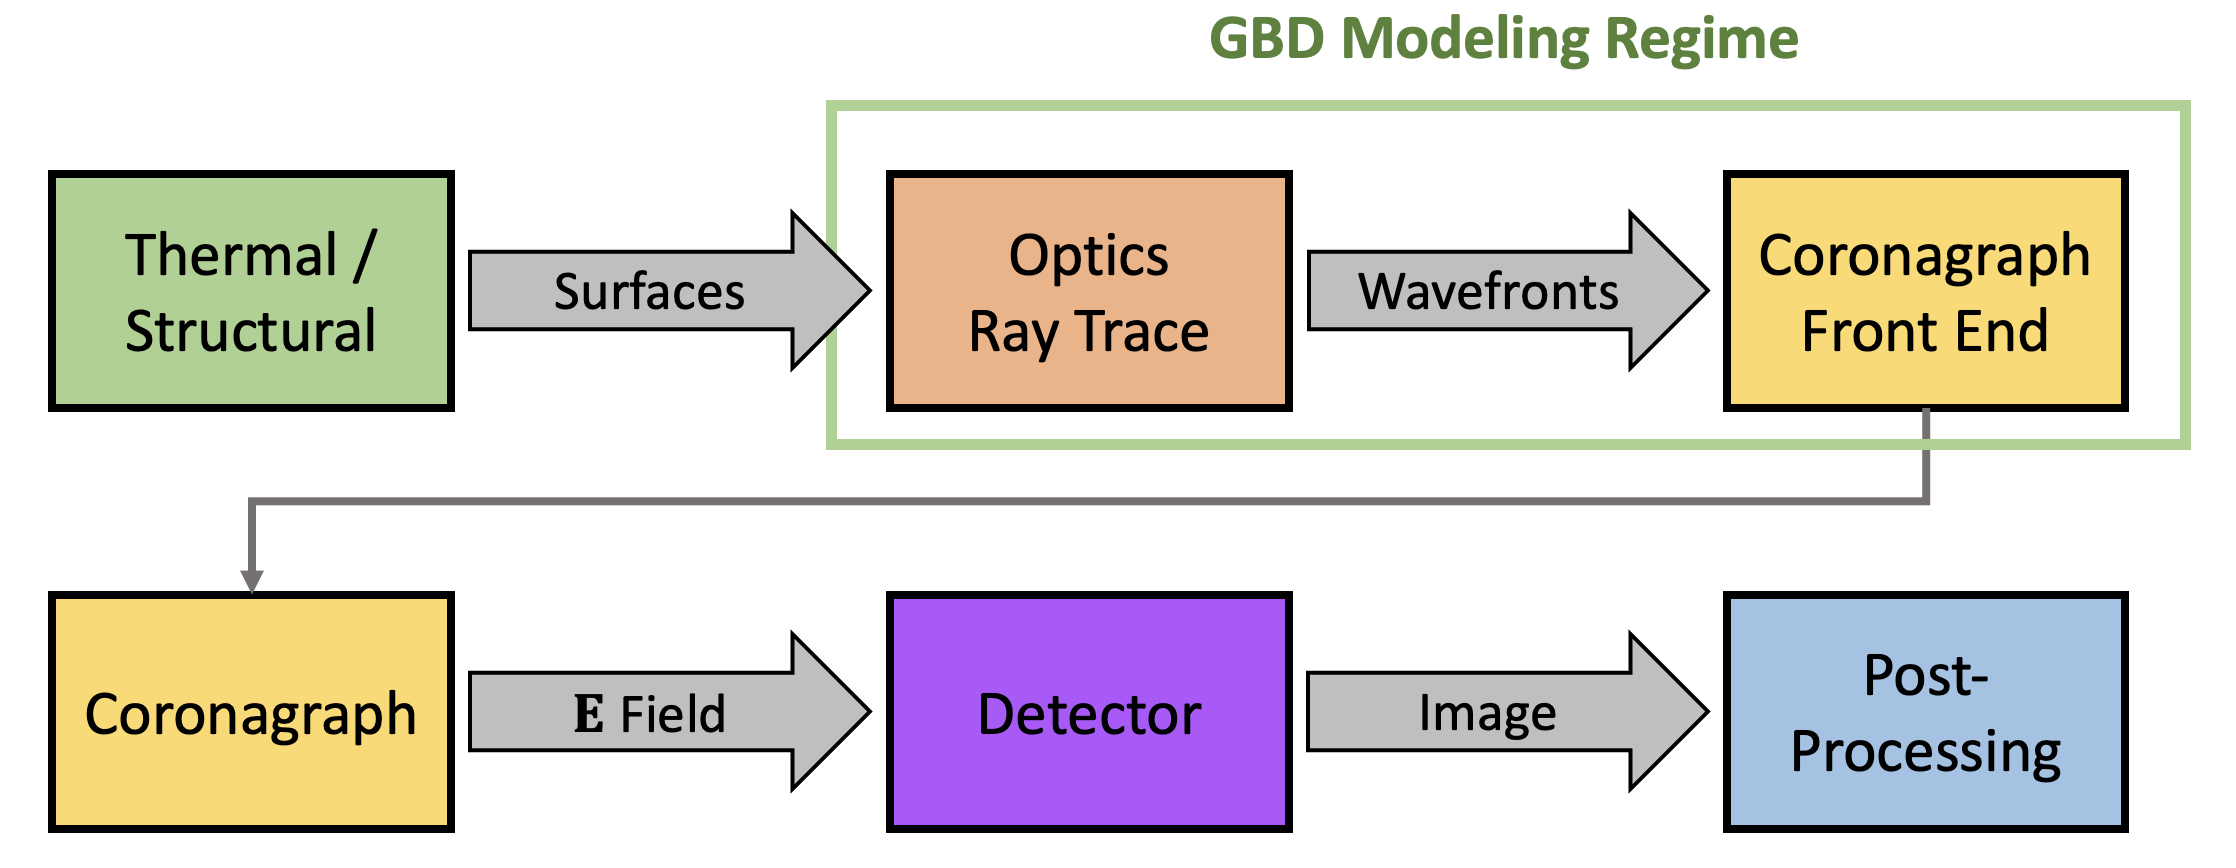
\includegraphics[width=\textwidth]{modeling_flow.png}
	\caption{Modeling flow inspired by the Structural Thermal Optical Performance (STOP) modeling process for the Roman Coronagraph \cite{Krist18}. This diagram illustrates the different modeling regimes required to create a simulated image of an observatory. We aim to further integrate this modeling pipeline by creating an open-source Gaussian Beamlet Decomposition platform to unify the ray trace model of the observatory with the diffraction model of the coronagraph.}
    \label{fig:modeling_flow}
\end{figure} 

To bridge the gap between commercial ray tracing engines and open-source physical optics propagation codes, we investigate the viability of a ray-based diffraction calculation called Gaussian Beamlet Decomposition (GBD) for \added{modeling} observatories with coronagraphs. \added{Traditionally, GBD operates using the complex ray tracing algorithm described in the works by Greynolds\cite{Greynolds86} and Harvey et al\cite{Harvey15}}. This technique has been previously implemented in FRED\cite{modeling_coherence_fred,Harvey15}, and possibly in CODE V\cite{bsp_in_codev}, but an exact method of its implementation in these software packages is not clearly available in the literature. \added{An alternative approach called the transfer matrix algorithm was recently developed to improve GBD's viability for precision diffraction simulation by Worku and Gross}\cite{Worku17,Worku:18,Worku19}. However, their implementation is not public and has not yet been formally evaluated as a tool to augment the modeling of astronomical observatories or high-contrast imaging instrumentation. \added{To formally evaluate GBD as a modeling tool for astronomical instrumentation, a complete algorithm for its implementation is derived in this manuscript.}

\subsection{Gaussian Beamlet Decomposition}
GBD is a method of physical optics propagation that approximates the propagated field as a finite sum of coherent Gaussian beams \added{that each propagate along a ray path}. This method has been implemented in optical design packages \cite{greynolds_ten_2020} to perform coherent calculations on non-paraxial systems. \added{The operating principle of GBD is to decompose the field in the entrance pupil of an optical system (Figure \ref{fig:gbd_essentials}a) into a finite set of Gaussian beams (Figure \ref{fig:gbd_essentials}b). Their coherent sum (Figure \ref{fig:gbd_essentials}c-d) approximates the initial field decomposition and can be propagated anywhere in the optical system along geometric ray paths.}

\begin{figure}[H]
    \centering
    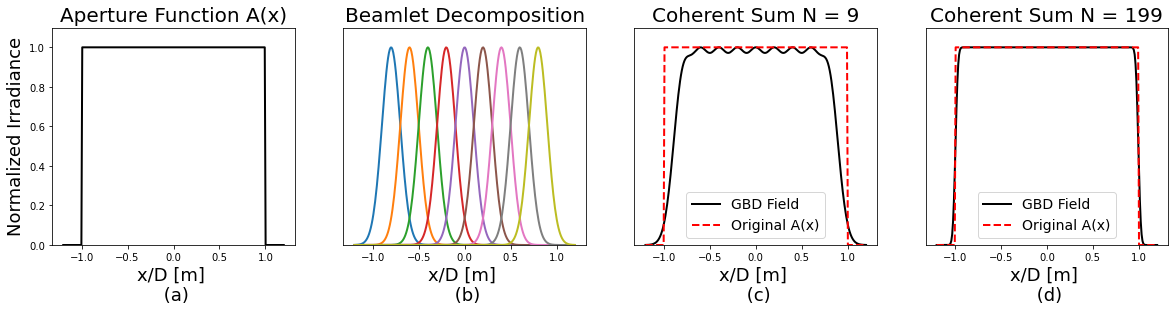
\includegraphics[width=\textwidth]{beamlet_decomposition_essentials.png}
    \caption{\added{Illustration of the operating principle of GBD in one dimension. The aperture function for traditional imaging systems is shown in (a) as a top-hat function. The decomposition of this function into a discrete set of Gaussian beams is shown in (b), which shows nine evenly-spaced Gaussian profiles before their coherent summation, which is shown in (c). The coherent sum (black) of these nine beamlets shows that the beamlets are incapable of perfectly reconstructing the original aperture function (dashed red), specifically the sharp edge and uniform amplitude. More beamlets are needed for a more accurate reconstruction, which is shown in (d) for 199 beamlets. The amplitude ripple has virtually vanished, and the field near the aperture edges is almost entirely recovered.}}
    \label{fig:gbd_essentials}
\end{figure}

\added{Under-sampling the field in the entrance pupil leads to artifacts in the decomposition. A characteristic amplitude ripple based on the period of the beamlet decomposition remains in the field. Due to the soft edges of the Gaussian beams, they cannot completely reconstruct the field of a sharp aperture edge. Using a larger number of smaller beamlets decreases the beamlet distribution period and increases the slope of the Gaussian beams, allowing for the mitigation of both of these effects (shown in Figure \ref{fig:gbd_essentials}d).}

\added{Upon decomposing the initial wavefront into a sufficient set of Gaussian beams, we can use their analytical linear propagation laws\cite{Siegman_1986} (described in \hyperref[sec:methods]{Section \ref{sec:methods}} of this manuscript) to compute the coherent field at any arbitrary plane in the optical system.} Fourier transform-based propagation methods derived from the Huygens-Fresnel principle typically assume the field is scalar and the optical system is paraxial \cite{goodman17}. This is usually appropriate for \added{stellar} coronagraphs, which operate on slowly focusing beams with diffraction-limited optics, \added{but may not be for next-generation observatories whose large apertures may necessitate relatively fast telescope optics}. 

GBD  compute\added{s} the same complex optical field without making the paraxial assumption across the \added{observatory}. Rather, the \added{coherent} field of  Gaussian beam\added{s} is derived from the ray data directly. Doing so imposes the paraxial assumption about a single beamlet \added{instead of the entire observatory}, which is a much less stringent approximation. Gaussian beams are technically infinite in extent, but extremely localized around the beam waist. Consequently, the contribution of the field very far from the Gaussian is negligible. \added{This locality} enables the \added{simulation of the} optical system to generally be non-paraxial\added{.} By making the diffraction calculation directly from ray data, GBD circumvents the need for \added{translating} the wavefront \added{to a physical optics propagator} and imposing the paraxial assumption on the optical system. Instead, the ray trace model can be directly integrated into the diffraction model. 

There are two main approaches that exist in the literature to implement GBD: the complex ray tracing method, and the transfer matrix method. The complex ray tracing method was recently described by Harvey et al\cite{Harvey15} in their seminal paper about implementing GBD in Photon Engineering's non-sequential ray tracing software FRED. This method traces waist and divergence rays to compute the complex field at the plane of interest using Arnaud's method of complex ray tracing\cite{arnaud_representation_1985,Greynolds86}. Through FRED, the complex ray tracing method has seen widespread use for nonparaxial coherent beam analysis.

\added{Another GBD approach, } the transfer matrix method was developed by Worku and Gross\cite{worku_vectorial_2017,Worku:18,Worku19} to mitigate GBD's inability to simulate sharp-edge diffraction and add new utility to the technique. This formulation of GBD works by computing the differential ray transfer matrix for a given ray path and then using that data to solve the Gaussian beam solution to the general Collins integral\cite{Collins:70}. Worku and Gross have leveraged the general Collins integral to provide alternative conditions to the Gaussian beam solution to modify the decomposition, such as truncated\cite{Worku19} and pulsed\cite{Worku:20} beamlet decomposition. The option of modifying the  beamlets to overcome the limitations of GBD makes the transfer matrix method extremely attractive for use in high-contrast imaging where preservation of high-spatial frequency content is important. Of particular interest are mirror segment gaps and opto-mechanical structures that obscure the primary mirror. Therefore, we elect to investigate Worku and Gross's transfer matrix method of GBD for the work presented in this manuscript. \added{Our goal is to publicize the transfer matrix method by developing an algorithm for its implementation, and then use it to characterize GBD's suitability for high-contrast imaging simulation. Our work can then be used as a platform with which to study the suitability of Worku and Gross' modified GBD in future investigations.}

\subsection{Hybrid Propagation Physics}
The ray-based nature of GBD introduces problems in modeling the electric field when the rays are vignetted. \added{Structure in the field where the initial decomposition occurs (typically, the entrance pupil) can be well-represented by Gaussian beams as long as the structure of interest is larger than the beamlets used in decomposition. Diffraction from structure in interemediate planes (between the pupil and focal planes) is challenging to represent if the beamlets diverge considerably. However, secondary beamlets can be traced from these intermediate structures to aid in the accuracy of the simulation\cite{Greynolds14}. At the focal plane of a diffraction-limited system, the rays are highly concentrated while the diffracted field spreads out considerably (e.g. the Airy disk). Because of GBD's reliance on ray tracing, it cannot represent diffraction from structure in the focal plane well without re-decomposing the field \cite{modeling_coherence_fred}.} For \added{the case of} a Lyot-type coronagraph all rays are vignetted at the focal plane mask (FPM) and the field decomposition is lost. To circumvent this we compute the field before the FPM with GBD and propagate it through the remaining coronagraph with traditional diffraction integrals, where we expect the low-order aberrations to be small and the paraxial assumption to be valid. This \emph{hybrid} method \added{(shown in Figure \ref{fig:hybridpropdiagram})} enables the user to alter the propagation physics for the electric field based on where it is the most appropriate; GBD will simulate the fast beams in the fore-optics and paraxial diffraction will propagate the field through the coronagraph imaging optics. \added{In practice, GBD would be used to propagate to the entrance pupil of the coronagraph for simulating systems with wavefront control, where it would then hand off the field to a paraxial diffraction model.}

\begin{figure}[H]
    \centering
    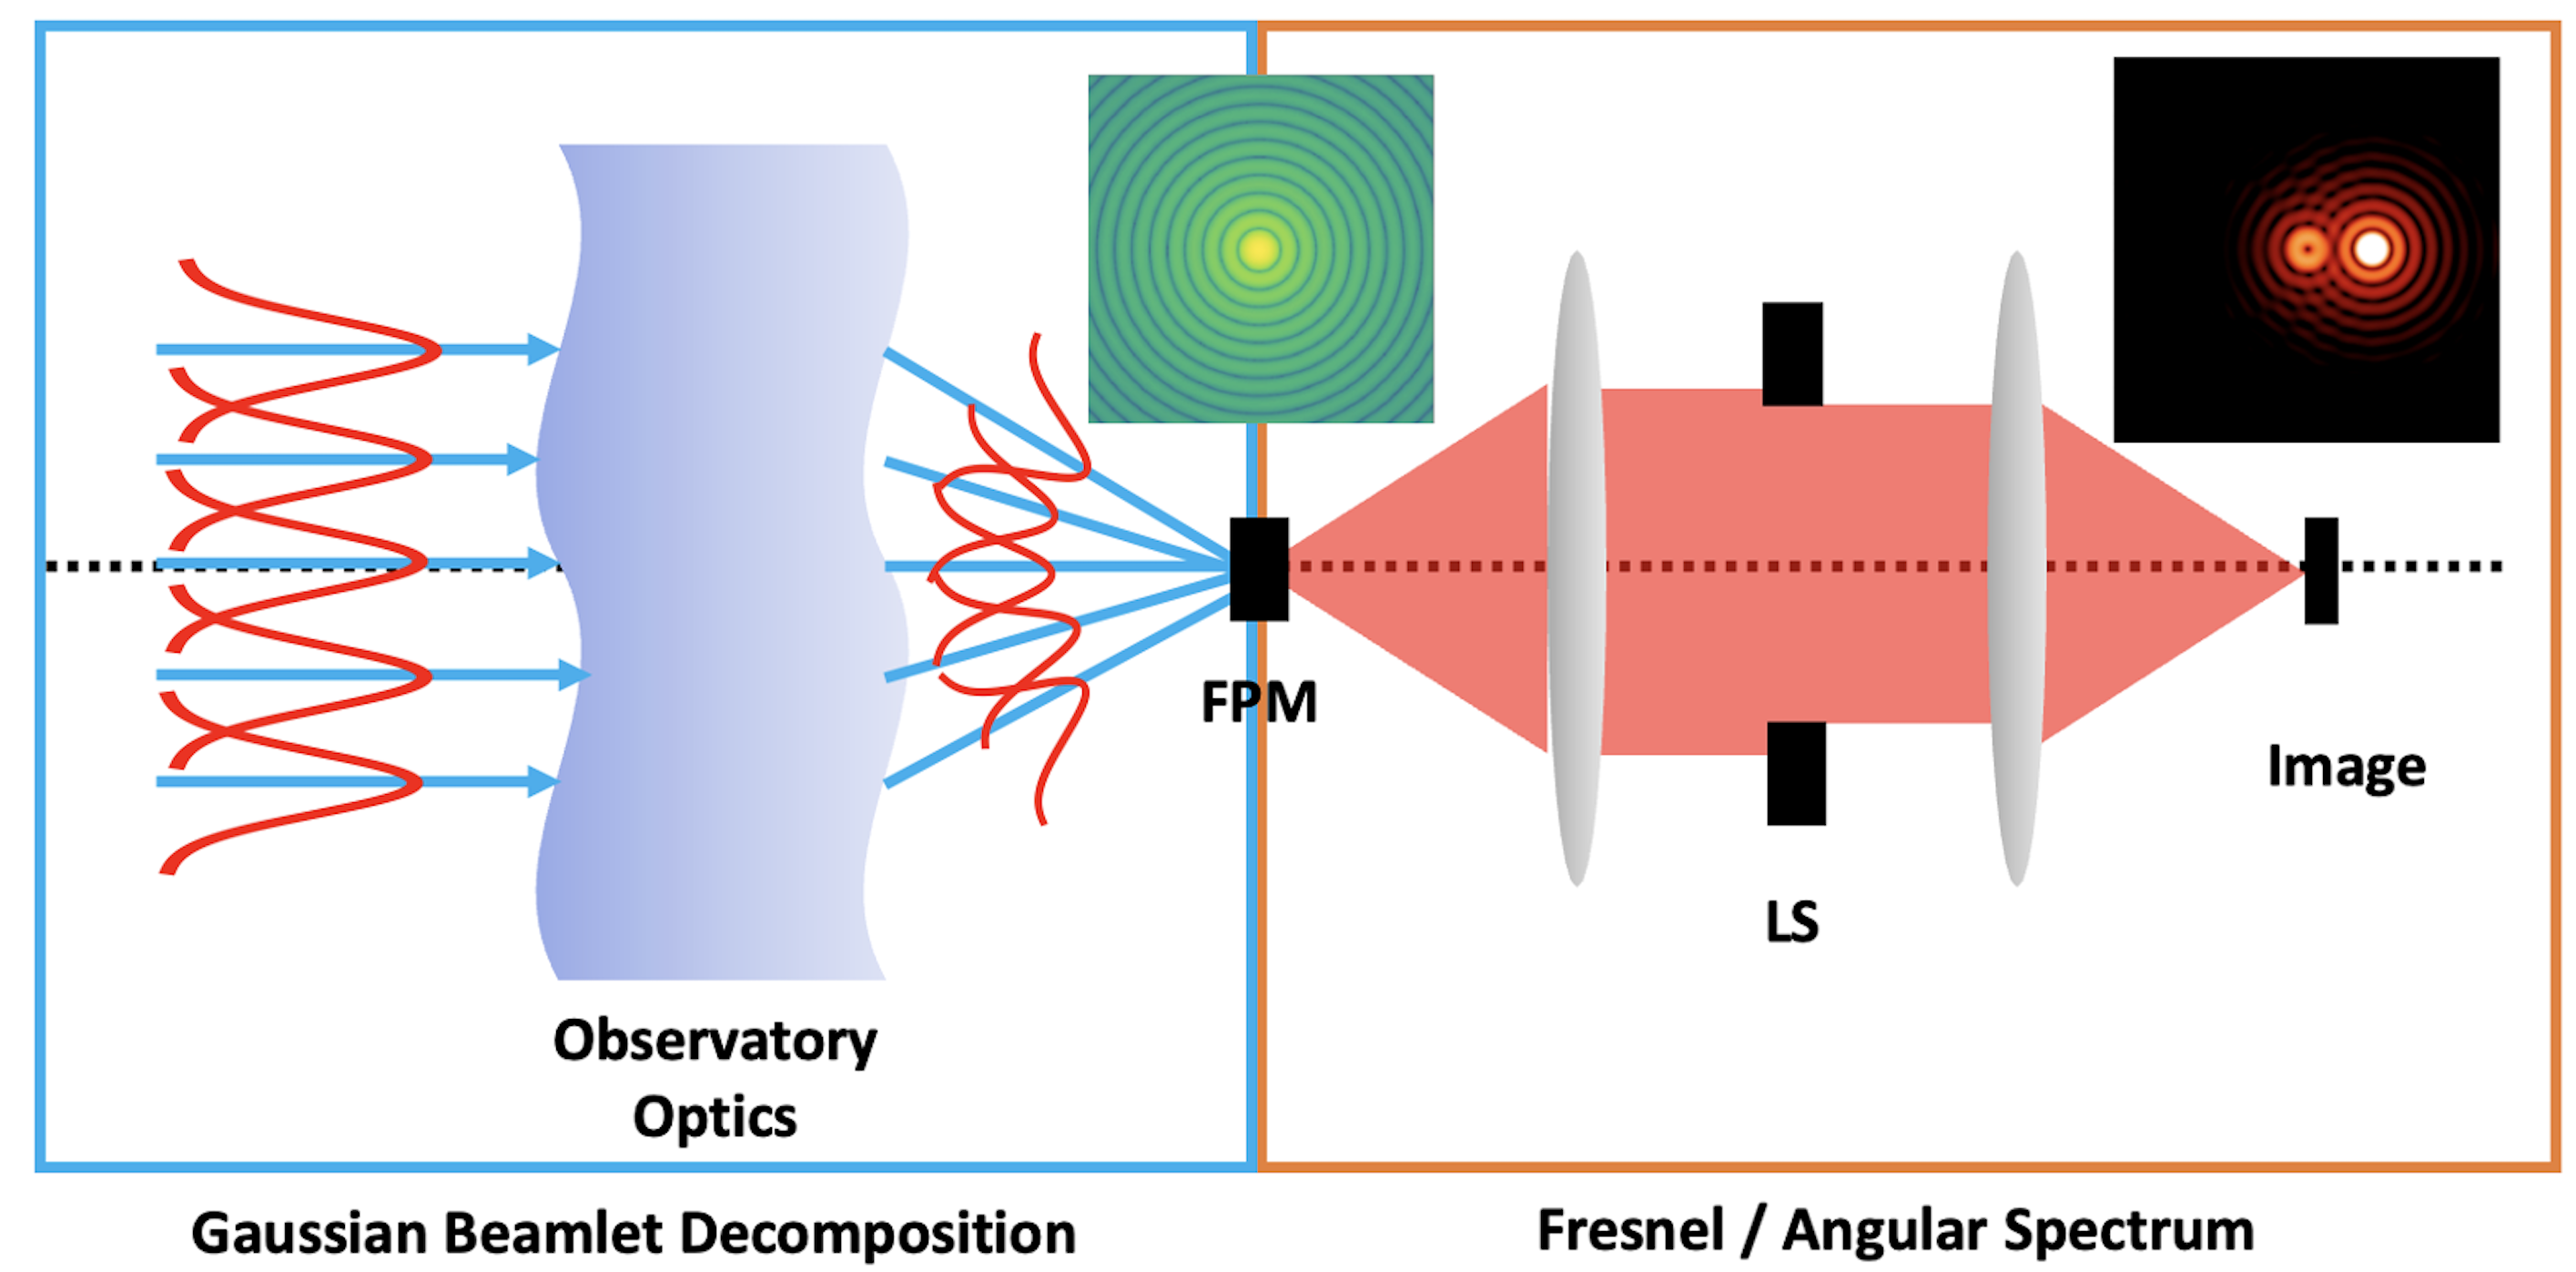
\includegraphics[width=\textwidth]{hybridprop2.png}
    \caption{Diagram demonstrating the hybrid propagation physics model. The observatory optics are best described by a ray-based propagation model, so GBD is used to compute the field at the image plane before the coronagraph focal plane mask (FPM). The field array is then passed to a paraxial diffraction model which propagates it past the FPM and through the remainder of the coronagraph. This propagation scheme permits the user to model the influence of the observatory optics non-paraxially, without losing accuracy after propagating past the focal plane mask.}
    \label{fig:hybridpropdiagram}
\end{figure}

The end result of such a model allows for direct integration of the ray trace model with the physical optics model, without imposing the paraxial approximation on the observatory. Like Fresnel and Fraunhofer diffraction, GBD is an approximation to diffraction physics. The decomposition of the field into Gaussian beams does not have an analytical solution. Therefore, undesirable artifacts can be introduced into the field if the decomposition is not well-understood and the sampling is insufficient\cite{Ashcraft2020}. To better understand the impact of a GBD PSF on high-contrast imaging simulations, we develop a hybrid propagation \added{model} to compare GBD to an equivalent Fraunhofer diffraction model.

To our knowledge, the transfer matrix method of GBD has not seen widespread implementation. Given its obvious benefits, we believe that this is because the transfer matrix method is not well-understood by the scientific community. We aim to remedy this by presenting a vectorizeable algorithm for the transfer matrix method, and open-sourcing our simulation platform for future investigators to use. This manuscript is the first work, to our knowledge, to provide the explicit mathematics of GBD \emph{and} provide our code as an object-oriented module for more widespread use. 

\added{Our GBD module was built in the Poke\cite{Ashcraft_poke_2022} Python package currently available on Github. Poke was originally developed to be a polarization ray tracing module to study the influence of polarization aberrations on astronomical coronagraphs\cite{anche_inprep}. For this study, we expanded its capabilities to include GBD. Poke operates by using ray tracer API's to trace a raybundle through every surface in the optical system. The relevant ray data is stored in a Rayfront object and can be loaded into a Python environment and interacted with independent of the ray tracer that generated the data. The Rayfronts can also be compiled into binary file types using the msgpack\cite{msgpack} package and distributed to any interested investigator, effectively open-sourcing the physical optics calculations done on ray data.}
\begin{figure}[H]
    \centering
    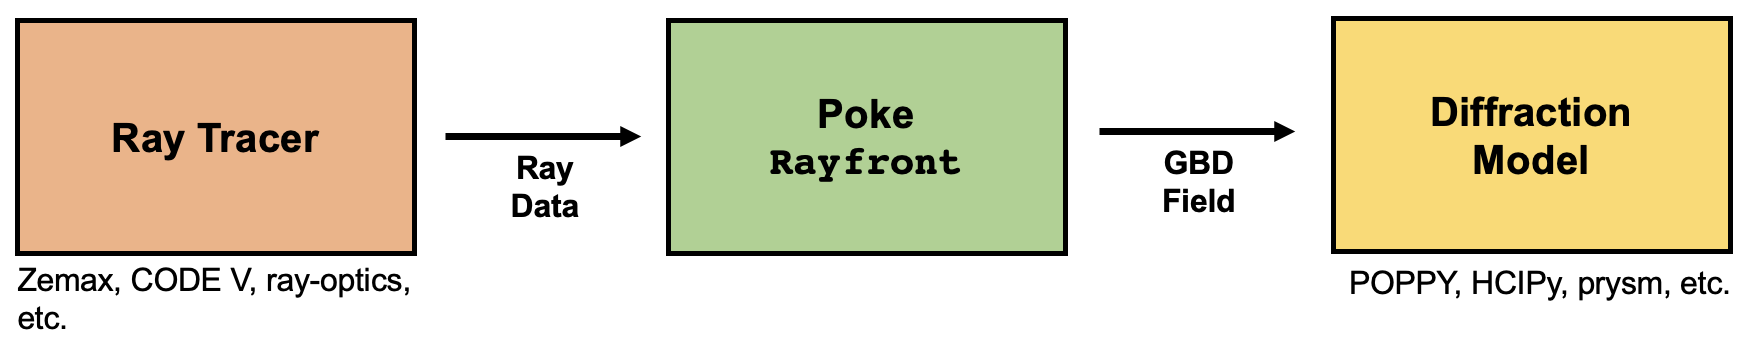
\includegraphics[width=0.9\textwidth]{poke_modeling_revised.png}
    \caption{\added{Illustration of Poke's use as an interface to open-source ray-based physical optics. Poke only requires an interface between a ray tracing engine (orange, left) to generate and save a Rayfront object, which includes all ray data necessary for the GBD calculation. Currently, Poke supports sequential systems in CODE V and Zemax, but we are working on adding support for open-source packages that have ray tracers, like ray-optics\cite{rayoptics}. The GBD field that Poke computes can then be sent to any open-source diffraction modeling package (yellow, right) to complete the hybrid propagation model.}}
    \label{fig:poke_modeling}
\end{figure}

\added{In this study we conduct ray traces in Zemax, which are then saved as a Poke Rayfront object. Poke performs the GBD simulations using the saved ray data to generate the field at the focal plane of the telescope. This data is exported to a coronagraph model built using HCIPy.}

In \hyperref[sec:methods]{Section \ref{sec:methods}} we outline the mathematics of Gaussian beam propagation and differential ray tracing used to perform GBD simulations. In \hyperref[sec:algorithm]{Section \ref{sec:algorithm}} we present the mathematical algorithm for the transfer-matrix method of GBD that we developed for this investigation. In \hyperref[sec:results]{Section \ref{sec:results}} we compare the results of observatory PSFs produced by GBD with one produced using traditional diffraction methods, and analyze the artifacts that remain in the field. In \hyperref[sec:conclusion]{Section \ref{sec:conclusion}} we assess the suitability of GBD for high-contrast imaging models and establish a roadmap for our module's continued development.